%##########################  CHAPER 6: APPLICATION  #######################

\chapter{Entwicklung der Anwendung}\label{kap:application}


Dieses Kapitel beschreibt die Realisierung der
Anwendung als autonomes Kamerasystem zur
Wildtiererkennung.

Zunächst werden dabei die verwendeten Hardwarekomponenten 
erläutert.

Im zweiten Abschnitt wird die Implementierung der 
Inferenz für eines der trainierten Modelle 
sowie einer geeigneten Kommunikationsmöglichkeit 
zur Übertragung der Daten beschrieben.


%-------------------------  SECTION 1: AUFBAU  ------------------------
\section{Hardware}\label{sec:aufbau}


Der Aufbau der Anwendung besteht aus einem, in Abbildung 
\ref{fig:raspberrypi} dargestellten \textit{Raspberry Pi 4},
auf dem der Programmcode ausgeführt wird,
sowie dem \textit{Neural Compute Stick 2}
 für die Inferenz, welcher über eine USB-Schnittstelle
mit dem \textit{Raspberry Pi} verbunden wird.

Zur Aufnahme der Bilder wurde das in 
Abbildung \ref{fig:rpicam} dargestellte 
\textit{Pi Kamera Modul},
mit einem \textit{5MP OV5647} Sensor der Marke \textit{Longrunner}
verwendet.
Dieses ermöglicht, durch mechanisches Zu und Abschalten
eines Infrarotfilters vor die Linse, zwischen Tag- und
Nachtsicht zu wechseln.
Der dafür verwendete Magnetschalter wird automatisch 
über einen Helligkeitssensor getriggert.
Im Infrarotmodus befindet sich der Filter nicht 
vor der Linse, sodass neben den elektromagnetischen 
Wellen des sichtbaren Lichts, auch die des 
langwelligeren Infrarotspektrums (850nm) 
auf die Linse treffen und verarbeitet werden können.

Zudem verfügt die Kamera über zwei Infrarot LEDs, 
sodass auch Aufnahmen in völliger Dunkelheit gemacht werden
können.
Der Vorteil dieser Infrarot-LEDs gegenüber normalen
LEDs liegt darin, 
dass die Tiere von keiner sichtbaren Lichtquelle 
gestört oder verscheucht werden.

Verbunden wird das Kameramodul über die \textit{\Gls{csi}}
Schnittstelle des \textit{Raspberry Pi's}.


\vspace{1cm}
%https://www.amazon.de/gp/product/B07R4JH2ZV/ref=ppx_yo_dt_b_asin_title_o01_s00?ie=UTF8&psc=1
\begin{minipage}{0.55\textwidth}
    \centering
    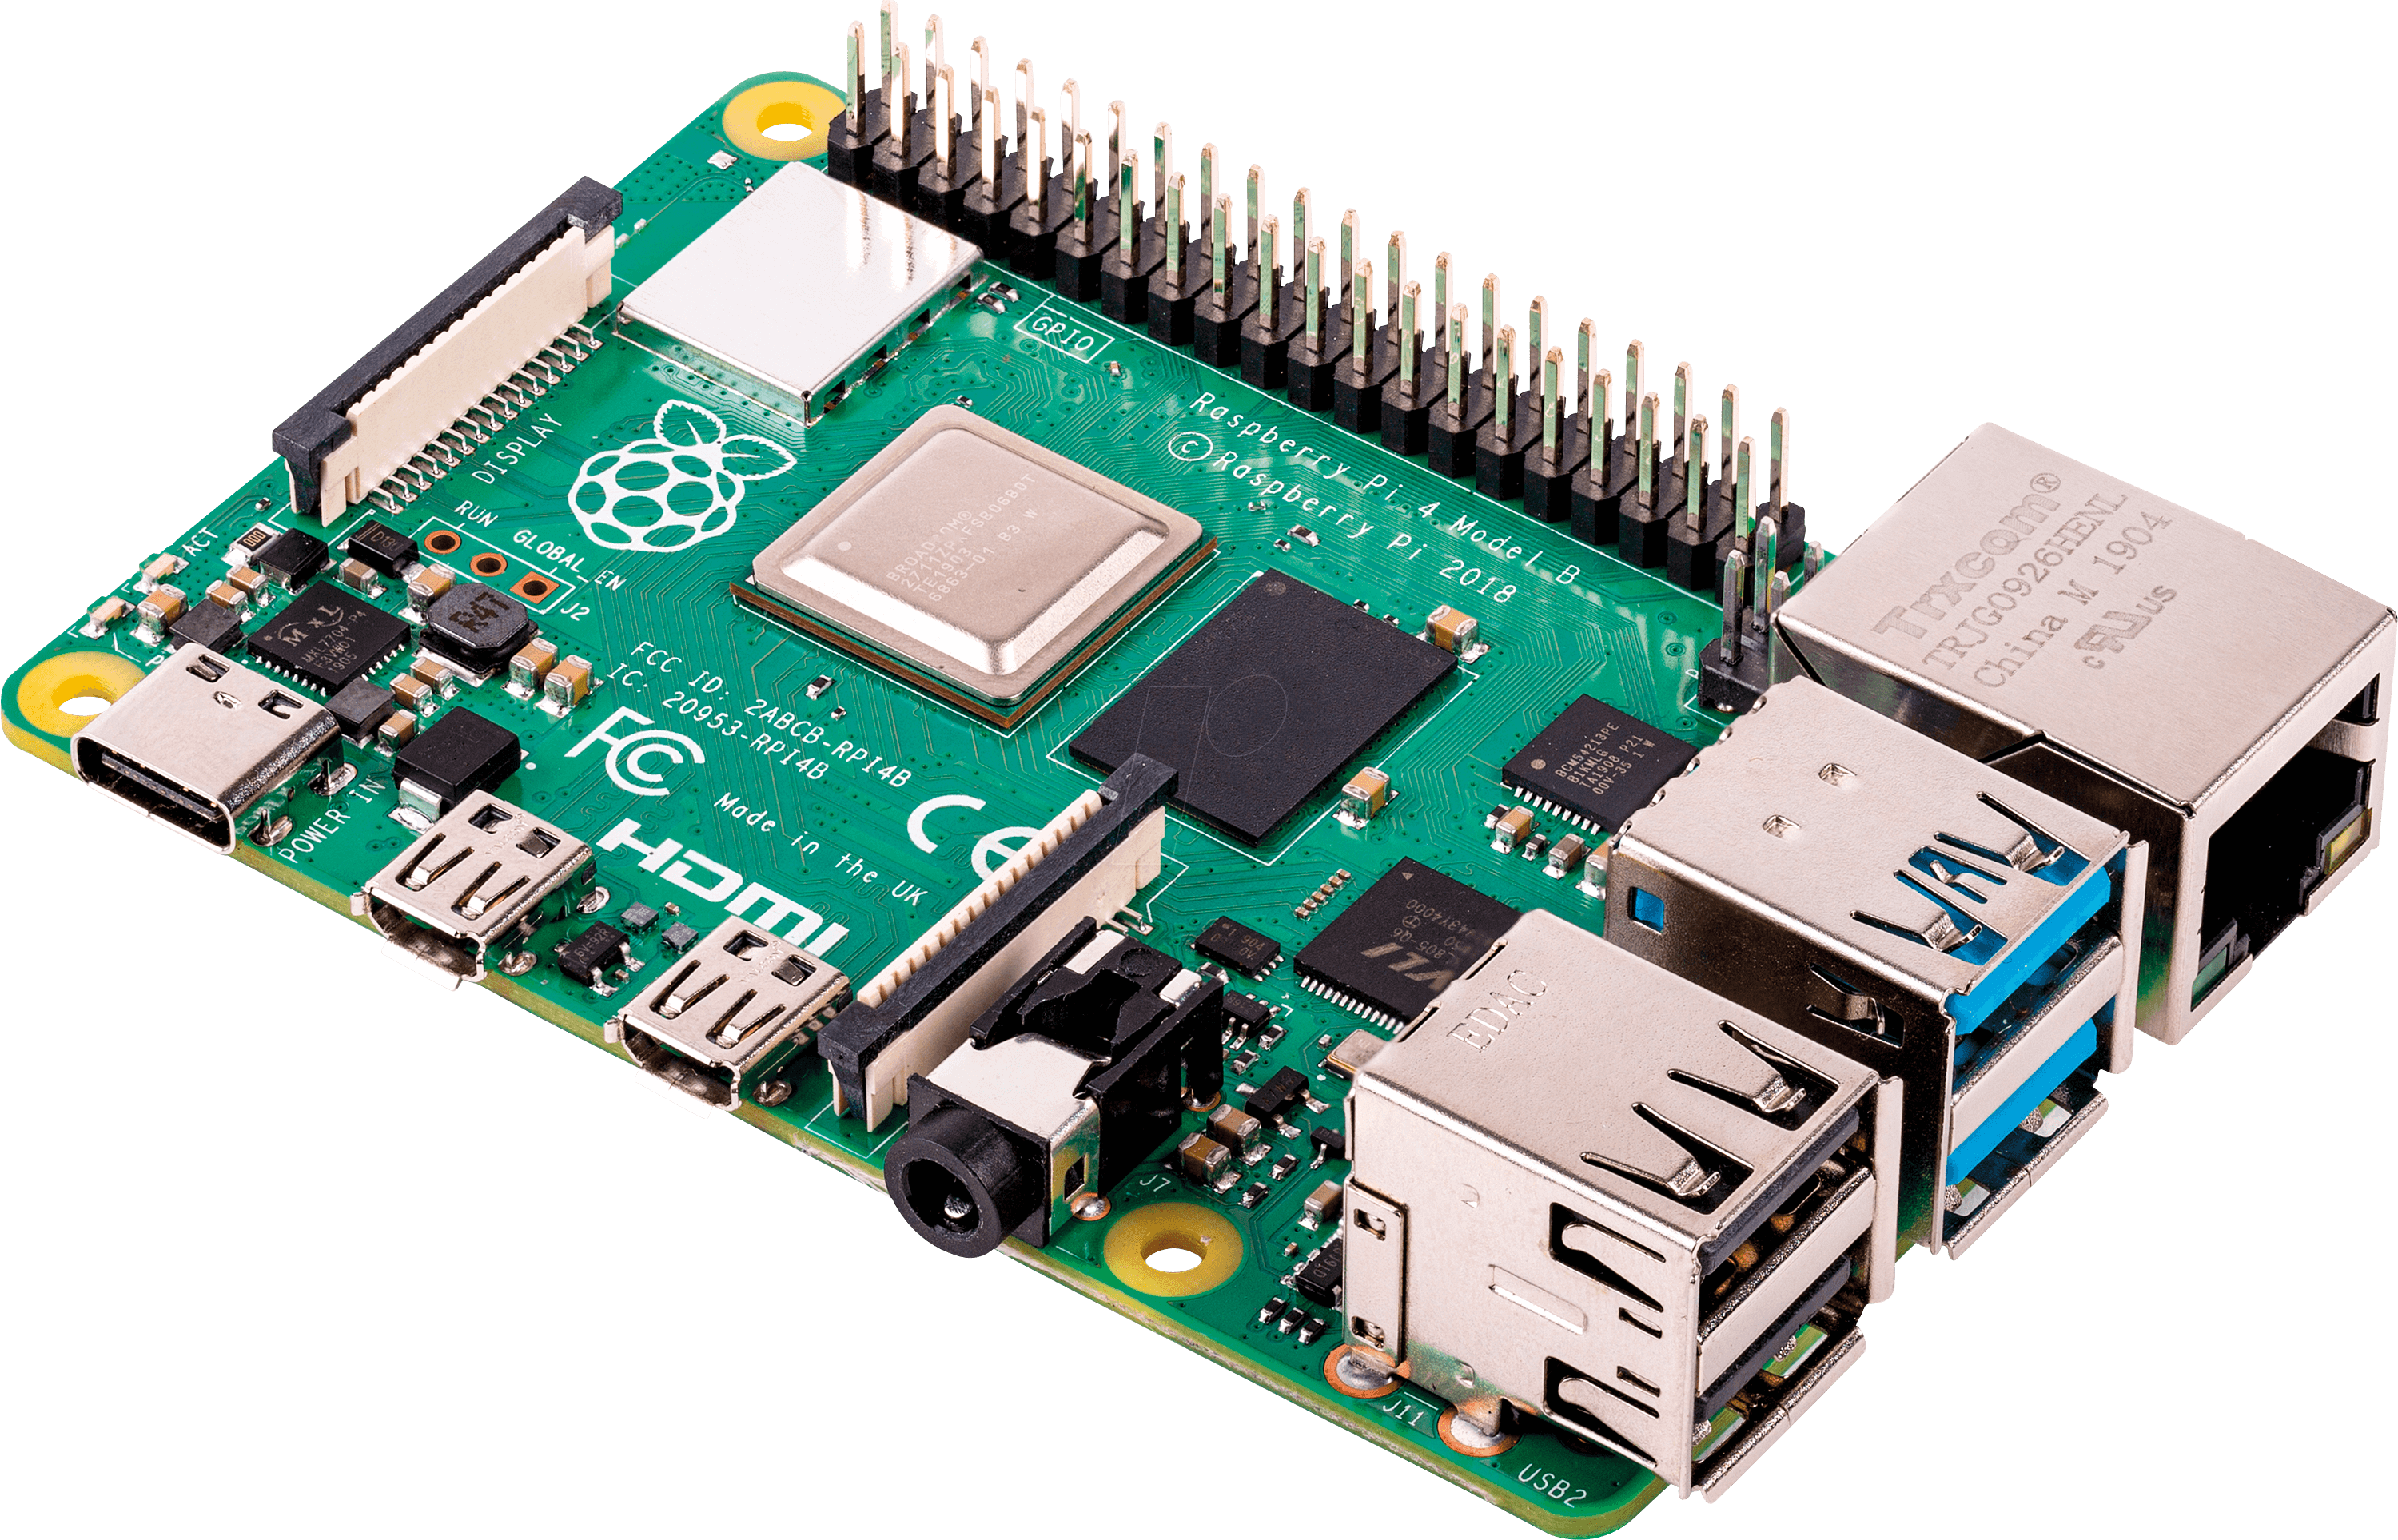
\includegraphics[width=0.8\textwidth]
    {./Bilder/raspberrypi_4.png}
    \captionof{figure}{Raspberry Pi 4}
    \label{fig:raspberrypi}
\end{minipage}
\begin{minipage}{0.45\textwidth}
    \centering
    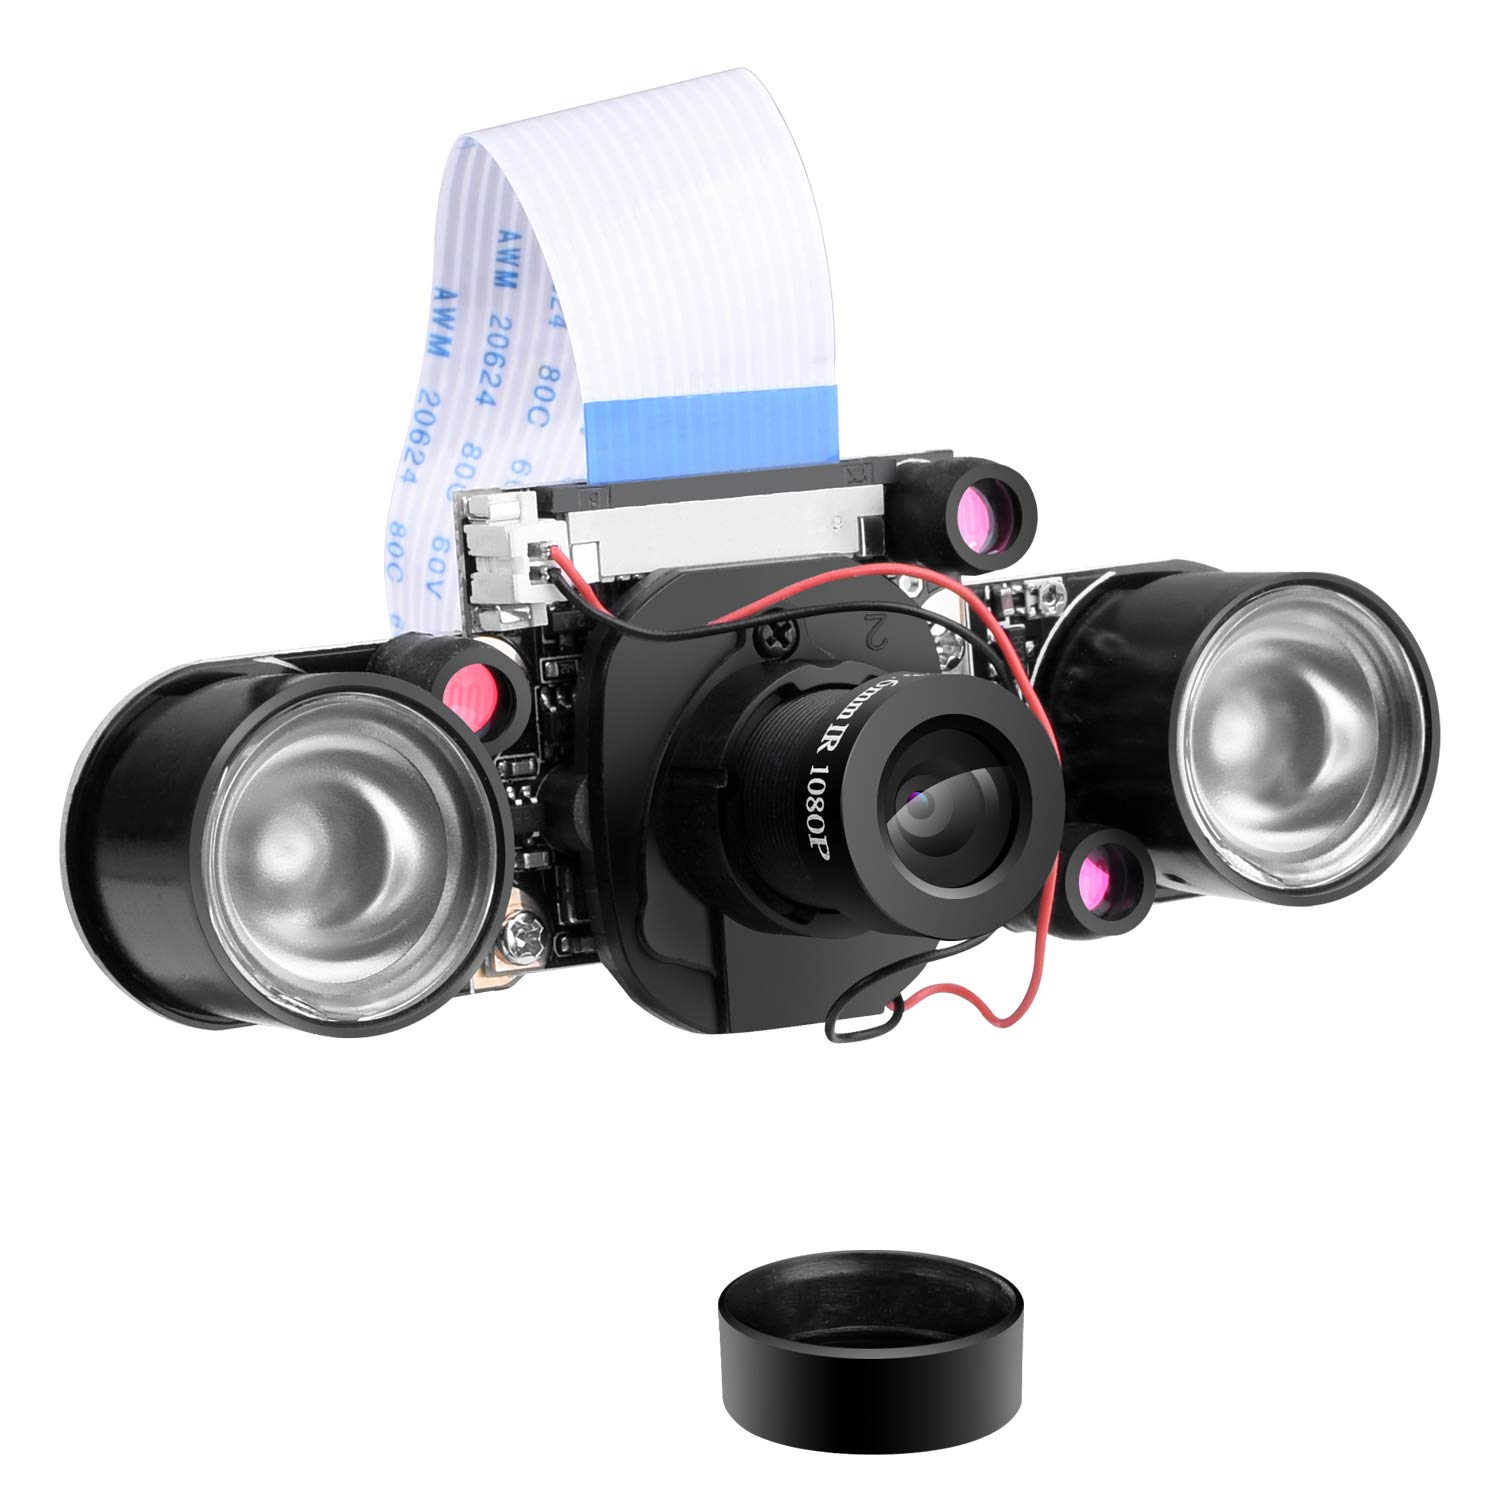
\includegraphics[width=0.8\textwidth]
    {longrunner.jpg}
    \captionof{figure}{Raspberry Pi Kameramodul mit Infrarot-LEDs}
    \label{fig:rpicam}
\end{minipage}
\vspace{1cm}


Des Weiteren wurde für eine mobile Internetverbindung 
der \textit{Huawei E3531 SurfStick} und zur
 Stromversorgung eine Powerbank verwendet.


\section{Software}

Die Implementierung der Applikation für den \textit{Raspberry Pi}
wurde mit Python vorgenommen. 
Dabei sind die Funktionalitäten zur Objekterkennung in
dem Script \textit{detection.py} 
und die Funktionalitäten zur Herstellung einer Verbindung
und Senden der Daten, in dem 
\textit{connection.py} Script definiert.

Der Kamera-Inputstream ist in einem \textit{main.py} Script 
implementiert, von dem aus auch die in Abbildung 
\ref{fig:class_diagram} 
dargestellten Klassen verwendet werden,
welche in \textit{detection.py} und \textit{connection.py}
enthalten sind.
\vspace{1cm}

\begin{minipage}{0.75\textwidth}
    \centering
    \underline{detection.py}
\end{minipage}
\begin{minipage}{0.25\textwidth}
    \centering
    \underline{connection.py}
\end{minipage}
\begin{figure}[H]
    \centering
    \begin{tikzpicture} 

    
    
            \umlclass{Motion}{ 
              statickBackground : np.array
              }{ 
              + detectMotion() : bool \\
              + resetBackground() : void
            }
        
            \umlclass[y=-4]{InferenceModel}{ 
                string : plugin
                strin : device
                }{ 
                + createExecInferModel() : ExecInferModel
              }
        
            \umlclass[y=-2, x=6]{ExecInferModel}{ 
                shape : ioBlob\\
                detected : array
                }{ 
                + inferFrames() : status \\
                \# status[0] num infered\\
                \# status[1] num detected\\
                \# status[2] num saved\\
                - save() : void
                }
        
    
        \umlclass[x=11, y=-2]{Connection}{ 
            string logindata
            }{ 
            + login() : bool \\
            + connect() : server, port\\
            + send() : bool\\
            + disconnect() : bool\\
            + sendEmail(email, text) : boiol
          }

    
    \end{tikzpicture}
            
    \caption{Klassendiagramm der Anwendung}
    \label{fig:class_diagram}
\end{figure}
\vspace{1cm}


Die Klasse \textit{Motion} dient der Erkennung von Bewegungen 
im Kamera-Inputstream, \textit{InferenceModel} und
\textit{ExecInferModel} realisieren die Inferenz 
eines trainierten Modells und die Klasse 
\textit{Connection} dient dem Aufbau einer
Verbindung zu einem anderen Gerät sowie dem Senden
der erkannten Bilder darüber.

Durch geeigneten Implementierung des Applikationsablaufes
sollte eine Möglichkeit gefunden werden, trotz 
der langsamen Inferenzzeit, mit dem Faster R-CNN
alle relevanten Frames, also die, in denen Tiere zu vermuten
sind, inferieren zu können.
Dafür wurde von der Annahme ausgegangen, dass zur Laufzeit der 
Anwendung, nicht durchgehend inferiert werden muss,
sich also zeitweise keine Tiere und damit auch keine 
Bewegungen vor der Kamera befinden.

Um Bewegungen feststellen zu können, 
wurde mithilfe der \textit{Library} \textit{OpenCV}
ein Bewegungsmelder implementiert.
Dieser speichert zu Beginn des Kamera-Streams einen 
Referenz-Frame ab, mit welchem alle weiteren Frames verglichen
werden.

Übersteigt der Abstand der einzelnen Pixelwerte im 
Graustufenbereich einen bestimmten
Threshold, wird dies als Bewegung gewertet.
Indem die Frames, die der Kamera-Stream permanent 
liefert, zunächst auf Bewegung überprüft werden, 
lässt sich unnötiges inferieren vermeiden,
was Zeit und Energie spart.
Frames, die Bewegung enthalten und aufgrund der langsamen 
Inferenzzeit des Faster R-CNN nicht sofort inferiert 
werden können, werden in einem Buffer zwischengespeichert
und in Phasen inferiert, zu denen keine Bewegung stattfindet.

Dafür musste der in Abschnitt \ref{sec:infertime} beschriebene
asynchrone Inferenzablauf dahingehend angepasst werden,
dass kein blockierendes Warten auf 
ein Inferenzergebnis stattfindet,
wodurch die Inferenz komplett zeitasynchron zu 
den Input-Frames ablaufen kann.
Der Gesamtablauf der Applikation ist in Abbildung 
\ref{fig:flowchart_appl} 
schematisch als Flussdiagram dargestellt.

\vspace{1cm}
\begin{figure}[H]
    \centering
    \tikzset{
    desicion/.style={
        diamond,
        draw,
        text width=4em,
        text badly centered,
        inner sep=0pt
    },
    block/.style={
        rectangle,
        draw,
        text width=10em,
        text centered,
        rounded corners
    },
    arrow/.style={
        draw,
        >=latex,
        ->
    }
}


\begin{tikzpicture}
    \node (A) [desicion] {entschei\\dung};
    \node (B) [block, below of=A, node distance=3cm, text width=5em] {bock};
    \node (C) [block, right of=A, node distance=0.5\textwidth] {noch ein\\bock};


    \draw[arrow] (A) --  node [left, fill=white!30] {yes} (B);
    \draw[arrow] (A) -- node [below, near end] {crap} (C); 
    \draw[arrow] (B) -| node [near start, fill=white] {yes} (C);

\end{tikzpicture}
    
    \caption{Schematischer Ablauf des Applikationscode}
    \label{fig:flowchart_appl}
\end{figure}
\vspace{1cm}


Wird in inferierten Frames mehrfach nichts 
erkannt, wird das Referenz-Frame des 
Bewegungsmelders durch ein aktuelles Frame ersetzt.

Erkannte Objekte werden in einer
Datenstruktur (Python Dictionary) zusammen 
mit Klassenname (cls), Wahrscheinlichkeit(p),
Anzahl an Erkennungen (N) sowie der
Bounding-Box-Koordinaten (Roi, (Region of Interest)) 
abgespeichert.


Nach einer bestimmten Anzahl 
an Erkennungen des selben Objekts, wird dieses 
als lokale Bilddatei abgespeichert und ein 
\textit{Send-Request} an das Main-Script zurückgegeben.

Dieses prüft dann, ob eine Verbindung zu einem 
anderen Gerät besteht, stellt diese gegebenenfalls her,
und sendet die lokal abgespeicherten Bilder.

Um nicht permanent die Verbindung zu einem PC aufrecht erhalten 
zu müssen, wird diese nach einer bestimmten Zeit ohne 
Bewegung getrennt. Dadurch wird das Datenvolumen 
des mobilen Internets nicht zu schnell aufgebraucht.

Im Folgenden werden die Funktionsweise der 
Inferenz sowie der Verbindungsaufbau 
genauer erklärt.


\subsection*{Inferenz}

Der im Abschnitt \ref{sec:infertime} beschriebene asynchrone
Inferenzablauf wurde dahingehend angepasst, dass eine beliebige
Anzahl an Inferenz-Requests verwendet werden kann 
und dass das Warten auf ein Inferenzergebnis
nicht mehr blockierend ist.
Dafür wurde der Timeout in der Wait-Funktion auf 
$0ms$ gesetzt.
Im Algorithmus \ref{code:infer_async_neu} ist 
der Inferenzablauf als Pseudocode dargestellt.

\begin{algorithm}[H]
    \caption{Asynchrone Inferenz, ohne Blockierung}
    \label{code:infer_async_neu}
    \begin{algorithmic}
    \WHILE{\TRUE}
    \STATE capture FRAMES
        \FOR{all InferRequests}
            %\STATE Status $\leftarrow$ \textbf{wait} for 
            % InferRequest
            \IF {\textbf{wait} for InferRequest \textbf{is} 0}
                \STATE Result $\leftarrow$ InferRequest.output
            \ENDIF
            \IF {Buffer \textbf{not} empty}
                \STATE preprocess InferRequest
                \STATE \textbf{start} InferRequest
            \ENDIF
            \IF{Result not NULL}
                \STATE process Result
            \ENDIF
        \ENDFOR
    \ENDWHILE
    \end{algorithmic}
\end{algorithm}    





\subsection*{Connection}

Um die Bilder mit erkannten Tieren an ein anderes Gerät 
z.B. einen PC senden zu können, musste eine Verbindung
hergestellt werden, die auch über verschiedene Netzwerke 
hinweg funktioniert.

Um unabhängig von Routerkonfigurationen und 
Firewalleinstellungen zu sein, wurde mithilfe des
Dienstes \textit{remot3.it} \cite{remot3}
eine Cloud-basierte Remote-Verbindung hergestellt.

Mit dieser war es möglich, eine \textit{Remote-Proxy} 
Verbindung über das \Gls{ssh} zu einem anderen Gerät 
herzustellen.
\vspace{1cm}

\begin{figure}[H]
    \centering
    \def\svgwidth{0.7\textwidth}
    \input{Bilder/diagram-connect.pdf_tex}
    \caption{Funktionsprinzip der Proxy-Verbindung}
    \label{fig:remoteit}
\end{figure}
\vspace{1cm}

Da die Daten vom \textit{Raspberry Pi} aus
 automatisch gesendet werden sollen, wurde der PC, an den 
sie Daten gesendet werden, als Remote-Gerät implementiert.

Gesendet wurden die Daten über das \Gls{scp}
welches \Gls{ssh} verwendet.

Dieses lässt sich über folgendes Kommando,
welches im \textit{connection.py}
Script ausgeführt wird, bedienen:
\begin{itemize}
    \item[\texttt{\$}] \texttt{scp -P port file.jpg 
    user@proxyadresse /zielpfad/file.jpg}
\end{itemize}

Server und Port werden dabei von \textit{remote.it}
generiert, \textit{file.jpg} ist das zu sendende Bild und
\textit{user} der Nutzername des Geräts,
an welches gesendet wird.
Um das Einloggen sowie den Verbindungsauf- und abbau 
über \textit{remote.it} zu einem Gerät automatisieren zu können,
bietet \textit{remote.it} eine \Gls{api}, mit der
über Post- und Get-Requests die Befehle dafür
programmatisch aufgerufen werden können.


Zusätzlich wurde eine Funktion implementiert,
die den Nutzer bei einer Erkennung automatisch 
per E-Mail benachrichtigt. Dafür wurde das
\Gls{smtp} verwendet.
